\documentclass[11pt,a4paper]{article}

\usepackage[margin=1in]{geometry}
\usepackage{amsmath,amssymb}
\usepackage{booktabs}
\usepackage{hyperref}
\usepackage[numbers,sort&compress]{natbib}
\usepackage{tikz}
\usepackage{pgfplots}
\usepackage{xcolor}
\usepackage{caption}
\usepackage{subcaption}
\usepackage{enumitem}
\usepackage{microtype}

\pgfplotsset{compat=1.18}
\usetikzlibrary{arrows.meta,positioning,shapes.geometric,calc,patterns}

\definecolor{cRed}{HTML}{c0392b}
\definecolor{cGreen}{HTML}{27ae60}
\definecolor{cBlue}{HTML}{2980b9}
\definecolor{cOrange}{HTML}{e67e22}
\definecolor{cGray}{HTML}{7f8c8d}

\hypersetup{
  colorlinks=true,
  linkcolor=cBlue,
  citecolor=cBlue,
  urlcolor=cBlue,
}

\title{No Threshold Is Safe: Oracle Bounds on\\
Similarity-Based Caching for Text-to-SQL}

\author{Ramakrishna Bobba\\
\texttt{https://github.com/rbobba/semantic-cache-inversion}}

\date{}

\begin{document}
\maketitle

% ============================================================
\begin{abstract}
Semantic caching for text-to-SQL reuses a stored query when a new question
is similar enough in embedding space. We show that this approach has a hard
ceiling: even an \emph{oracle} per-entry threshold---one that picks the
best possible threshold for every cached entry individually---recovers at
most 6--17\% of reusable queries at zero false reuse, across 15 embedding
models from nine publishers (2021--2026). The information needed to
separate safe reuse from unsafe reuse is not in the similarity score.

A structured guard that matches on an extracted signature---operation,
measure, grouping and exclusion---achieves 77--100\% correct reuse on 480
human-written questions across four analytics domains, with two extractor
vendors. This guard design is prior art \cite{rathore2026cogni,
bindschaedler2026semantic}; our contribution is testing it on held-out
human wording with pre-registered decision rules.

We also document an extraction hazard not previously reported: excluded
values (``everything except travel'') are silently dropped 4--40\% of the
time by a small extraction model (4\% in healthcare, 35--40\% in the other
three domains), while the same value is extracted
correctly when included. The residual risk is date semantics: rolling
periods and explicit date ranges defeat every design tested.

Dataset, code and all model outputs:
\url{https://github.com/rbobba/semantic-cache-inversion}
\end{abstract}

% ============================================================
\section{Introduction}

Semantic caching reduces latency and cost in text-to-SQL systems by reusing
a stored SQL query when a new natural-language question is close enough in
embedding space \cite{bang2023gptcache, singh2026semantic}. The key
decision is the similarity threshold: too low and the cache misses; too
high and it serves wrong SQL silently.

The practitioner's assumption is that better threshold tuning, or a learned
per-entry threshold \cite{schroeder2026vcache, wang2025category}, will make
the cache safe. Several recent systems already go further: COGNI gates
reuse on entity overlap, intent and polarity checks
\cite{rathore2026cogni}; Bindschaedler matches on exact OLAP intent
signatures \cite{bindschaedler2026semantic}; AWS validates extracted
parameter formats against template placeholders \cite{brukau2026aws}. But
the failure mode these systems address has been asserted, not measured:
COGNI states that period-differing queries ``often exceed 0.95 cosine
similarity'' without running an embedding baseline
\cite{rathore2026cogni}, and Bindschaedler argues that similarity caches
``cannot distinguish'' total from average revenue without quantifying it
\cite{bindschaedler2026semantic}.

This paper contributes three results:

\begin{enumerate}[leftmargin=*,itemsep=2pt]
\item \textbf{An oracle bound.} We compute the ceiling for \emph{any}
      threshold-based similarity method: even with a perfect per-entry
      threshold, correct reuse at zero false reuse is at most 6--17\%
      (Section~\ref{sec:oracle}). This closes the threshold-tuning
      direction, including learned methods such as vCache
      \cite{schroeder2026vcache}.

\item \textbf{An extraction hazard.} Excluded values are dropped by the
      extractor 4--40\% of the time, while the same value is extracted
      correctly when included (Section~\ref{sec:exclusion}). This
      asymmetry has not appeared in prior error taxonomies.

\item \textbf{Guard tested on held-out human wording.} We evaluate the
      structured-guard design of \citet{rathore2026cogni} and
      \citet{bindschaedler2026semantic} on 480 questions written by people
      who never saw the templates, with two extractor vendors and
      pre-registered decision rules (Section~\ref{sec:guard}).
\end{enumerate}

\noindent
We do not propose a new caching method. The guard design is prior art. Our
contribution is the measurement and the honest reporting of where it
breaks.

\begin{figure}[t]
\centering
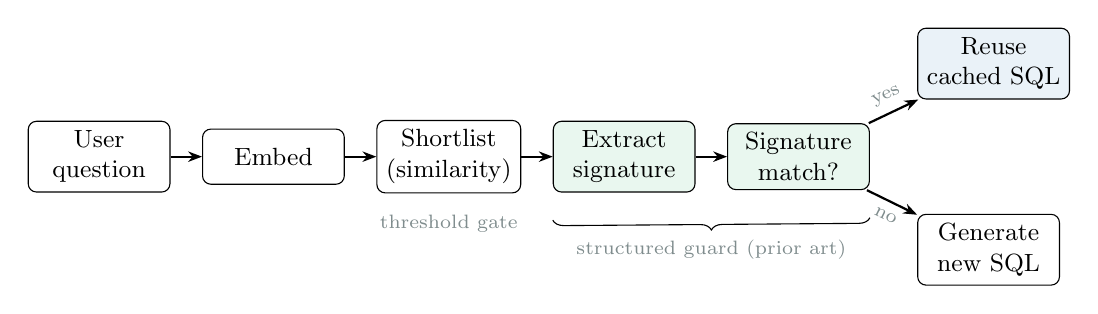
\begin{tikzpicture}[
  node distance=0.4cm,
  box/.style={draw, rounded corners=3pt, minimum height=0.7cm,
              minimum width=1.8cm, font=\small, align=center},
  arr/.style={-{Stealth[length=5pt]}, thick},
  lbl/.style={font=\scriptsize, text=cGray},
]
  \node[box] (q) {User\\question};
  \node[box, right=of q] (emb) {Embed};
  \node[box, right=of emb] (short) {Shortlist\\(similarity)};
  \node[box, right=of short, fill=cGreen!10] (ext) {Extract\\signature};
  \node[box, right=of ext, fill=cGreen!10] (match) {Signature\\match?};
  \node[box, above right=0.3cm and 0.6cm of match, fill=cBlue!10] (reuse) {Reuse\\cached SQL};
  \node[box, below right=0.3cm and 0.6cm of match] (gen) {Generate\\new SQL};

  \draw[arr] (q) -- (emb);
  \draw[arr] (emb) -- (short);
  \draw[arr] (short) -- (ext);
  \draw[arr] (ext) -- (match);
  \draw[arr] (match) -- node[lbl, above, sloped] {yes} (reuse);
  \draw[arr] (match) -- node[lbl, below, sloped] {no} (gen);

  \node[lbl, below=0.15cm of short] {threshold gate};
  \draw[decorate, decoration={brace, mirror, amplitude=4pt}]
    ($(ext.south west)-(0,0.35)$) -- ($(match.south east)-(0,0.35)$)
    node[lbl, midway, below=4pt] {structured guard (prior art)};
\end{tikzpicture}
\caption{A semantic cache pipeline with a structured guard. The
similarity shortlist is a necessary but insufficient pre-filter; the guard
checks that the extracted parameters match the cached entry's signature.
This design is described by \citet{rathore2026cogni} and
\citet{bindschaedler2026semantic}; we measure its performance on held-out
human wording.}
\label{fig:architecture}
\end{figure}

% ============================================================
\section{Setup}
\label{sec:setup}

\paragraph{Task.} A text-to-SQL semantic cache stores
(question, SQL) pairs. When a new question arrives, the cache embeds it,
finds the most similar stored question, and---if similarity exceeds a
threshold---returns the stored SQL without calling the language model. A
\emph{correct} reuse returns the same SQL intent the new question needs; a
\emph{false} reuse returns SQL for a different intent.

\paragraph{Models.} We test 15 embedding models from nine publishers:
sentence-transformers (MiniLM, mpnet), BAAI (bge), intfloat (e5),
Mixedbread (mxbai), Snowflake (arctic), Qwen (Qwen3-0.6B), Google
(text-embedding-004, gemini-embedding-001), OpenAI (text-embedding-3-small,
3-large), and Voyage (voyage-3-large, 3.5, 4). Release years span
2021--2026.

\paragraph{Domains.} Four analytics domains: personal finance, retail,
healthcare operations and IT support. Each domain has 125--145 cached questions
generated from domain-specific templates with controlled parameter
variations (period, entity, measure and exclusion).

\paragraph{Human questions.} 480 questions written by three volunteers who
never saw the templates, across all four domains (120 per domain). Each
question targets a specific cached template but uses the writer's own
wording.

\paragraph{Extractors.} Two LLM-based extractors: Google Gemini
(gemini-3.1-flash-lite) and OpenAI (gpt-6-luna), each run three times for
stability.

\paragraph{Pre-registration.} Every hypothesis, decision rule and
prediction was committed before its run. Three stages recorded SHA-256
hashes of their pre-registration text. Predictions that turned out wrong
are kept in place, not edited. The full record is in the repository's
\texttt{STUDY\_LOG.md}.

% ============================================================
\section{The Oracle Bound}
\label{sec:oracle}

The central question for threshold-based caching is: if we could pick the
\emph{best possible} threshold for every cached entry independently---with
full knowledge of every query that will arrive---how much correct reuse
could we recover at zero false reuse?

\paragraph{Definition.} For each cached entry, find the highest
threshold that still produces zero false reuse---the best any system
could do with perfect foresight. Set every entry to its own best
threshold. This is the oracle per-entry method.
Formally, for entry~$c_i$, define
$\tau^*_i = \max\{\tau : \text{no false reuse of } c_i \text{ at threshold } \tau\}$.
Any method that learns a per-entry threshold \cite{schroeder2026vcache}
is bounded above by this oracle, because the oracle has perfect knowledge
of the query distribution.

\paragraph{Results.} Table~\ref{tab:oracle} shows the oracle bound across
15 models on the finance dataset (128 cached entries, 53.2\% of incoming
queries have a reusable match).

\begin{table}[t]
\centering
\caption{Correct reuse at zero false reuse (\%). The oracle per-entry
threshold is the ceiling for any threshold-based similarity method. The
template cache with oracle parameters shows what extracted structure
recovers. Four representative models are shown; the full table (15 models)
is in the appendix.}
\label{tab:oracle}
\small
\begin{tabular}{@{}lcccc@{}}
\toprule
Model (year) & Global & Oracle & Template & Possible \\
             & thresh. & per-entry & (oracle params) & \\
\midrule
MiniLM-L6-v2 (2021)     &  0.8 &  7.1 & 97.3 & 53.2 \\
bge-base-en-v1.5 (2023)    &  0.5 &  8.1 & 97.3 & 53.2 \\
text-emb-3-large (2024)  &  1.2 &  9.8 & 97.3 & 53.2 \\
gemini-emb-001 (2025)    &  0.2 & 10.2 & 100.0 & 53.2 \\
voyage-4 (2026)          &  6.3 & 16.8 & 97.3 & 53.2 \\
\midrule
\textit{Range (all 15)}  & \textit{0.2--6.3} & \textit{6.4--16.8}
                          & \textit{96.2--100.0} & \textit{53.2} \\
\bottomrule
\end{tabular}
\end{table}

\begin{figure}[t]
\centering
\begin{tikzpicture}
\begin{axis}[
  ybar,
  bar width=14pt,
  width=\columnwidth,
  height=5.5cm,
  ymin=0, ymax=105,
  ylabel={Correct reuse at zero false reuse (\%)},
  ylabel style={font=\small},
  symbolic x coords={Global,Oracle per-entry,Template match},
  xtick=data,
  xticklabel style={font=\small, align=center},
  ytick={0,20,40,60,80,100},
  yticklabel style={font=\small},
  point meta=explicit,
  nodes near coords={\pgfmathprintnumber\pgfplotspointmeta},
  nodes near coords style={font=\scriptsize,
    /pgf/number format/.cd, assume math mode, fixed, precision=1},
  every node near coord/.append style={anchor=south},
  legend style={at={(0.02,0.98)}, anchor=north west, font=\scriptsize},
  clip=false,
  enlarge x limits=0.25,
]

\addplot[fill=cRed!70, draw=cRed]
  coordinates {(Global,0.9) [0.9] (Oracle per-entry,10.2) [10.2] (Template match,0) []};

\addplot[fill=cGreen!70, draw=cGreen]
  coordinates {(Global,0) [] (Oracle per-entry,0) [] (Template match,97.3) [97.3]};

\draw[dashed, thick, cGray] (axis cs:Global,53.2) -- (axis cs:Template match,53.2)
  node[anchor=south east, font=\scriptsize, text=cGray] {reusable (53.2\%)};

\legend{Similarity threshold (median of 15 models),
        Extracted structure (oracle params)}
\end{axis}
\end{tikzpicture}
\caption{The oracle bound. Even a perfect per-entry threshold recovers
only $\sim$10\% of reusable queries (median across 15 models). Template
matching with extracted parameters recovers 97\%. The dashed line shows
the fraction of queries that \emph{should} be reusable. The gap between
the oracle bar and the dashed line cannot be closed by any
threshold-based method.}
\label{fig:oracle}
\end{figure}

\paragraph{Why the bound is so low.} The bound is low because the
similarity ordering is \emph{inverted}: a one-word period swap (``this
year'' $\to$ ``last year'') scores higher than any rewording of the same
question. In the finance domain, the period swap outscores the best
rewording for 78--100\% of cached entries, in all 15 models (comparison~A
in the study log). There is no threshold to find because the wrong query
is not between the right queries---it is above them.

\paragraph{Implications.} This bound applies to any method that makes a
reuse decision based solely on a scalar similarity score per entry. It
covers global thresholds, per-entry thresholds
\cite{schroeder2026vcache}, category-aware thresholds
\cite{wang2025category}, and LLM-as-judge methods that score similarity
\cite{singh2026krites}. The bound does \emph{not} apply to methods that
examine the embedding vector's internal structure or that use additional
extracted features---those are the structured guards of
Section~\ref{sec:guard}.

% ============================================================
\section{The Exclusion-Drop Asymmetry}
\label{sec:exclusion}

During the extraction experiments, we observed an asymmetry not documented
in prior error taxonomies \cite{rathore2026cogni, bindschaedler2026semantic,
jivani2026tecod}: excluded values are dropped far more often than included
values.

\paragraph{The finding.} When a question says ``everything except travel,''
the extractor should produce \texttt{exclusion=travel}. With
gemini-3.1-flash-lite, it drops the exclusion in 4--40\% of such
questions (4\% in healthcare, 35--40\% in the other three domains). The same category is extracted correctly 100\% of the time when
the question asks \emph{for} it rather than \emph{excluding} it
(Table~\ref{tab:exclusion}).

\begin{table}[t]
\centering
\caption{Exclusion-drop rates by domain (gemini-3.1-flash-lite, pooled
across three runs). The included-value column is the same categories in
non-negated questions.}
\label{tab:exclusion}
\small
\begin{tabular}{@{}lccc@{}}
\toprule
Domain & Excluded dropped & Included wrong & Difference [95\% CI] \\
\midrule
Finance     & 39/111 (35\%) & 0/111 (0\%) & 0.35 [0.21, 0.49] \\
Retail      & 39--40/105 (37--38\%) & 0/104 (0\%) & 0.37--0.38 \\
Healthcare  & 5/112 (4\%)  & 0/114 (0\%) & 0.045 [0.009, 0.080] \\
IT support  & 45--46/116 (39--40\%) & 3/122 (2\%) & 0.36--0.37 \\
\bottomrule
\end{tabular}
\end{table}

\paragraph{Why it matters.} A dropped exclusion turns ``spending except
travel'' into ``all spending''---a plausible-looking wrong answer with no
error signal. The result is that similarity correctly identifies the right
template, the guard correctly matches the signature, and the cache still
serves wrong SQL because the exclusion was lost during extraction.

\paragraph{Prompt sensitivity.} An unrelated change to the extraction
prompt's period section doubled the exclusion-drop rate in one experiment
(Section~13 of the study log). This suggests the asymmetry is a side effect of how the model
distributes attention across the prompt, not a reliable model property.

\paragraph{Caveat.} This is primarily a small-model effect.
Gemini-3.5-flash (a frontier model at higher cost) dropped zero excluded
values in finance, retail and healthcare. The hazard is real for
cost-sensitive deployments that use smaller extraction models.

% ============================================================
\section{Guard Results on Human Questions}
\label{sec:guard}

The structured guard extracts a signature from the incoming question---
operation (sum, count, average), measure (what is being measured),
grouping (how results are grouped) and exclusion (what is excluded)---and
reuses a cached entry only if the signature matches. This is the design
described by \citet{rathore2026cogni} and
\citet{bindschaedler2026semantic}. We test it on 480 human-written
questions with two extractor vendors.

\paragraph{Results.} Table~\ref{tab:guard} shows correct reuse and wrong
reuse rates by domain and vendor. For comparison, an exact-key cache
(reuse only when the question string matches exactly) achieves 0--4\%
correct reuse.

\begin{table}[t]
\centering
\caption{Guard performance on 480 human-written questions, by domain and
extractor vendor. Correct reuse: fraction of meaning-preserving questions
served from cache. Wrong reuse: fraction served with a wrong template.
Ranges span three repeat runs $\times$ four embedders.}
\label{tab:guard}
\small
\begin{tabular}{@{}lcccc@{}}
\toprule
Domain & \multicolumn{2}{c}{Correct reuse (\%)} & \multicolumn{2}{c}{Wrong reuse (\%)} \\
\cmidrule(lr){2-3} \cmidrule(lr){4-5}
       & Gemini & OpenAI & Gemini & OpenAI \\
\midrule
Finance    & 100      & 98--99 &  0     & 0.4   \\
Retail     & 94--100  & 85--88 & 0--5.7 & 2.1--2.6 \\
Healthcare & 90--98   & 91--100 & 0.4--7.6 & 0--8.8 \\
IT support & 88--98   & 77--87 & 0--11.8 & 0--13.4 \\
\midrule
\multicolumn{5}{l}{\textit{Exact-key baseline: 0--4\% correct reuse across all domains}} \\
\bottomrule
\end{tabular}
\end{table}

\paragraph{Where the guard leaks.} Every wrong reuse on held-out wording
was traced to its cause:

\begin{itemize}[leftmargin=*,itemsep=1pt]
\item \textbf{Retail:} ``units sold'' was read as a sum in 52 extractions
      and a count in 59 extractions. When the extractor guesses wrong, the
      signature matches the wrong template.
\item \textbf{Healthcare:} ``clinic visits'' was labeled ``inbound'' in
      83 of 114 extractions. The remaining errors are from templates that
      share a signature by design (visits $\leftrightarrow$ no-shows).
\item \textbf{IT support:} ``top teams'' and ``top services'' have the
      same extracted signature by design. No extraction error is needed
      for this false match.
\end{itemize}

\paragraph{Comparison with prior evaluations.} COGNI reports zero false
hits on 200 queries constructed by its authors
\cite{rathore2026cogni}. Bindschaedler reports 82\% hits with zero false
hits on 1,395 queries including 10 manually authored paraphrases per
intent \cite{bindschaedler2026semantic}. Our evaluation differs in that
the question writers never saw the templates, and the results show
domain-specific failure modes that constructed queries may not surface.

% ============================================================
\section{What the Guard Cannot Catch}
\label{sec:residual}

Two classes of queries defeat every design tested in this study:

\begin{enumerate}[leftmargin=*,itemsep=2pt]
\item \textbf{Rolling dates.} ``The past year'' could mean the rolling 12
      months or the calendar year. The extracted period label is the same;
      the SQL is different. Neither similarity nor the signature
      distinguishes them.

\item \textbf{Explicit date ranges.} ``From January~15 to March~1'' is a
      specific interval that no relative label captures. The guard's
      signature has no slot for arbitrary date ranges.
\end{enumerate}

\noindent
Relative period labels (``this month,'' ``last quarter'') \emph{did}
remove every period error in extraction: zero errors in 15,411
extractions across all domains and runs. The fix is effective for the
common case but does not cover the long tail of date expressions.

% ============================================================
\section{Related Work}
\label{sec:related}

\paragraph{Semantic caching.} GPTCache \cite{bang2023gptcache} established
the embed-search-reuse pattern. MeanCache \cite{gill2025meancache} argues
existing caches give ``unacceptable false hit-and-miss rates'' and adds
context chains. vCache \cite{schroeder2026vcache} learns per-entry
thresholds; our oracle bound (Section~\ref{sec:oracle}) shows this
direction has a low ceiling for text-to-SQL. Category-aware thresholds
\cite{wang2025category} and LLM judges \cite{singh2026krites} also operate
on scalar similarity and fall under the same bound.

\paragraph{Structured guards.} COGNI \cite{rathore2026cogni} gates reuse
on conjunctive checks including entity overlap, intent and polarity.
Bindschaedler \cite{bindschaedler2026semantic} matches on exact OLAP
intent signatures. AWS \cite{brukau2026aws} validates extracted parameter
formats. Our study tests this design class on held-out human wording and
reports the domain-specific failure modes.

\paragraph{Near-miss queries.} TeCoD \cite{jivani2026tecod} finds that
cosine-threshold template selection performs poorly (63.5\% selection
accuracy on BIRD) and that ``the bulk of the error is due to the wrong
literal generation even after matching with the correct template.'' This
is consistent with our finding that template matching works but parameter
extraction is fragile.

\paragraph{Embedding blind spots.} Negation blindness in text embeddings
\cite{cao2025negation} is the mechanism behind our exclusion-drop
finding: the extractor's embedding-based attention gives less weight to
negation cues. CacheAttack \cite{zhang2026cacheattack} shows that
similarity locality conflicts with collision resistance, achieving 86\%
hijack rates. The theoretical argument that embeddings can discard the
information needed for valid cache hits is made by
\citet{zhang2026validity}.

\paragraph{Operational evaluation.} \citet{baral2026operational} argue
that ``models with the highest PR-AUC are often the worst in
operation''---threshold-invariant metrics mask operational failures. Our
reporting of correct reuse at fixed false-reuse budgets follows their
recommendation.

% ============================================================
\section{Limitations}
\label{sec:limitations}

\textbf{Scope.} Four analytics domains, one language (English), one
question shape (single-table aggregation queries). Multi-table joins,
subqueries and non-aggregation queries are not covered.

\textbf{Extractors.} Both extractors are frontier LLMs (Gemini flash-lite,
OpenAI gpt-6-luna). Traditional NER or smaller models may behave
differently. The exclusion-drop asymmetry was not tested on non-LLM
extractors.

\textbf{No production traffic.} All questions are either template-generated
(synthetic) or volunteer-written (human). Neither represents the
distribution of a production analytics tool. The guard's performance on
production traffic is an open question.

\textbf{Model breadth vs.\ depth.} We tested 15 models but all on the
same task. Four or five models spanning open and commercial publishers
would have supported the same conclusions. The additional 10 models
confirm universality but the marginal value of each additional model is
small.

\textbf{Pre-registration.} Pre-registration is evidence of discipline, not
proof of correctness. It prevents post-hoc threshold tuning and selective
reporting, but the pre-registered decision rules themselves could be poorly
chosen.

% ============================================================
\section{Conclusion}

The threshold-tuning direction for text-to-SQL semantic caching has a hard
ceiling. An oracle per-entry threshold recovers at most 6--17\% of
reusable queries at zero false reuse, across 15 embedding models spanning
five years. The information needed to distinguish safe from unsafe reuse is
not in the similarity score.

Structured guards that match on extracted signatures---a design proposed by
\citet{rathore2026cogni} and \citet{bindschaedler2026semantic}---achieve
77--100\% correct reuse on human-written questions. The guard leaks are
domain-specific and traceable to extraction ambiguity, not to the guard
design itself.

The residual risk is date semantics. Rolling periods and explicit date
ranges produce wrong SQL that no design tested here catches. This is the
open problem.

\paragraph{Reproducibility.} The dataset (480 human-written questions,
four domains), all model outputs, extraction results and evaluation code
are available at
\url{https://github.com/rbobba/semantic-cache-inversion}.
The \texttt{verify\_claims.py} script recomputes every number cited in the
study log from the files on disk.

\bibliographystyle{plainnat}
\bibliography{references}

% ============================================================
\clearpage
\appendix
\section{Full Oracle Bound Table}
\label{app:oracle}

Table~\ref{tab:oracle-full} shows the oracle bound for all 15 models on
the finance dataset.

\begin{table}[h]
\centering
\caption{Correct reuse at zero false reuse (\%), all 15 models.}
\label{tab:oracle-full}
\small
\begin{tabular}{@{}lcccc@{}}
\toprule
Model (year) & Global & Oracle & Template & split\_full \\
             & thresh.\ & per-entry & (oracle) & (oracle) \\
\midrule
all-MiniLM-L6-v2 (2021)           & 0.8 &  7.1 & 97.3 & 21.3 \\
all-mpnet-base-v2 (2021)           & 1.8 &  6.6 & 96.2 & 21.5 \\
e5-base-v2 (2023)                  & 0.9 &  8.1 & 97.3 & 21.4 \\
bge-base-en-v1.5 (2023)            & 0.5 &  8.1 & 97.3 & 21.8 \\
text-embedding-3-small (2024)      & 0.2 &  6.4 & 97.3 & 21.4 \\
text-embedding-3-large (2024)      & 1.2 &  9.8 & 97.3 & 22.5 \\
mxbai-embed-large-v1 (2024)        & 0.6 & 10.6 & 100.0 & 22.6 \\
snowflake-arctic-embed (2024)      & 2.1 & 10.7 & 97.3 & 22.4 \\
text-embedding-004 (2024)          & 0.5 &  9.3 & 97.3 & 24.2 \\
text-emb-004 SemSim (2024)         & 1.1 & 11.0 & 97.3 & 27.3 \\
voyage-3-large (2025)              & 1.1 & 14.4 & 100.0 & 27.2 \\
voyage-3.5 (2025)                  & 0.6 & 11.4 & 100.0 & 24.9 \\
gemini-embedding-001 (2025)        & 0.2 & 10.2 & 100.0 & 32.0 \\
Qwen3-Embedding-0.6B (2025)        & 1.1 & 11.2 & 97.3 & 21.5 \\
voyage-4 (2026)                    & 6.3 & 16.8 & 97.3 & 30.0 \\
\midrule
\textit{Range} & \textit{0.2--6.3} & \textit{6.4--16.8}
               & \textit{96.2--100.0} & \textit{21.3--32.0} \\
\bottomrule
\end{tabular}
\end{table}

\section{Comparison A Across Domains}
\label{app:comp-a}

Comparison~A measures: for each cached entry, does the period swap score
higher than the best rewording? Table~\ref{tab:comp-a} shows the rate
across four domains for representative models.

\begin{table}[h]
\centering
\caption{Comparison~A: fraction of cached entries where the period swap
outscores the best rewording (higher = worse for caching). Four
representative models shown; all 15 behave similarly.}
\label{tab:comp-a}
\small
\begin{tabular}{@{}lcccc@{}}
\toprule
Model & Finance & Retail & Healthcare & IT support \\
\midrule
bge-base-en-v1.5    & 0.875 & 0.922 & 0.945 & 0.960 \\
text-emb-3-large    & 0.945 & 0.984 & 0.972 & 0.992 \\
gemini-emb-001      & 0.898 & 0.930 & 0.931 & 0.984 \\
voyage-4            & 0.789 & 0.836 & 0.793 & 0.912 \\
\bottomrule
\end{tabular}
\end{table}

\section{AUC on Human Questions}
\label{app:auc}

Table~\ref{tab:auc} shows the AUC for separating rewordings from period
changes on 480 human-written questions. All 15 models cluster near the
coin-toss line (0.50).

\begin{table}[h]
\centering
\caption{AUC for rewording vs.\ period-change separation on human
questions. An AUC of 0.50 is chance. The pre-registered decision rule
required all upper confidence bounds below 0.80; this holds.}
\label{tab:auc}
\small
\begin{tabular}{@{}lcc@{}}
\toprule
Model & AUC & 95\% CI \\
\midrule
all-MiniLM-L6-v2      & 0.526 & [0.449, 0.608] \\
all-mpnet-base-v2      & 0.522 & [0.443, 0.604] \\
bge-base-en-v1.5       & 0.580 & [0.507, 0.655] \\
e5-base-v2             & 0.581 & [0.506, 0.662] \\
Qwen3-Embedding-0.6B   & 0.595 & [0.519, 0.677] \\
Snowflake Arctic       & 0.561 & [0.486, 0.639] \\
mxbai-embed-large      & 0.545 & [0.474, 0.619] \\
text-embedding-004     & 0.524 & [0.449, 0.602] \\
text-emb-004 SemSim    & 0.559 & [0.480, 0.639] \\
gemini-embedding-001   & 0.559 & [0.480, 0.634] \\
text-embedding-3-small & 0.581 & [0.505, 0.665] \\
text-embedding-3-large & 0.594 & [0.513, 0.681] \\
voyage-3-large         & 0.595 & [0.520, 0.672] \\
voyage-3.5             & 0.550 & [0.475, 0.628] \\
voyage-4               & 0.595 & [0.528, 0.671] \\
\bottomrule
\end{tabular}
\end{table}

\end{document}
